\chapter{Generative Adversarial Network}
\begin{onehalfspace}
    A GAN comprises two components, a generator $(G)$ and a discriminator $(D)$. 
    The goal of the generator model is to produce new data similar to the required 
    one. The discriminator's task is to classify the data presented to it as real or 
    fake. Real data belong to the original dataset, and fake data are those 
    forged by the generator. The generative model competes against its adversary, 
    the discriminative model that learns to determine whether a sample is from the 
    model distribution or the data distribution.    
\section{Analogy}
    Generative networks can be thought of as a team of counterfeiters trying 
    to produce fake currency notes and use it without being caught by the 
    police. Here discriminative networks play the role of police trying to 
    detect fake currency. Initially, both the police and counterfeiters are not 
    very experienced, but as the game between them progresses, both parties 
    master what they were doing.  The game continues until the fake currency 
    notes produced by the counterfeiters are indistinguishable from real 
    currency.

\section{A Mathematical Model}

    Assume that the generator represented by the neural network 
    \(G(z, \theta_{1})\) converts the input noise \(z\) into the required output 
    space. Conversely, a second neural network \(D(x, \theta_{2})\) represents 
    discriminator, and it calculates the probability that x came from the real 
    dataset. Here, $\theta_{1}$ and $\theta_{2}$ represents the weights that 
    describe each neural network.

    The discriminator is trained to classify the input data as either real or 
    fake. The weights of the discriminator are updated so that it maximizes the 
    probability that real images from the database are classified as real and 
    minimizes the probability that images generated by G are classified as fake. 
    The loss function used for the discriminator maximizes \(D(x)\) and minimizes 
    \(D(G(z))\). 

    The generator's weights are trained to maximise the probability that it can 
    fool the discriminator using the images it generates. The loss function 
    maximizes \(D(G(z))\).

    \begin{figure}[h]
        \centering
        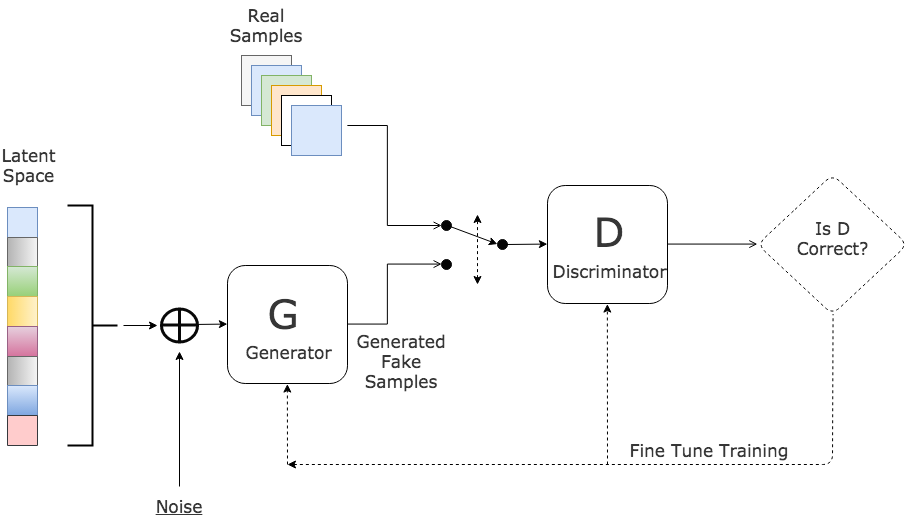
\includegraphics[width=0.8\linewidth]{generative-adversarial-network.png}
        \caption{Generative Adversarial Network Architecture}
        \label{fig:gans}
    \end{figure} 

    Figure \ref{fig:gans} shows a visual representation of the high level 
    overview of GANs discussed in this section.
    During training, the generator is trying to maximize \(D(G(z))\) and 
    discriminator is trying to minimize \(D(G(z))\).  Thus we can think of the 
    scenario as the generator and discriminator as playing a minimax game.
\section{Applications of GAN}
    \subsection{Generate Anime characters}
    Game development and animation production are expensive and hire many production artists for relatively routine tasks. GAN can auto-generate and colorize Anime characters.
    \begin{figure}[h]
        \centering
        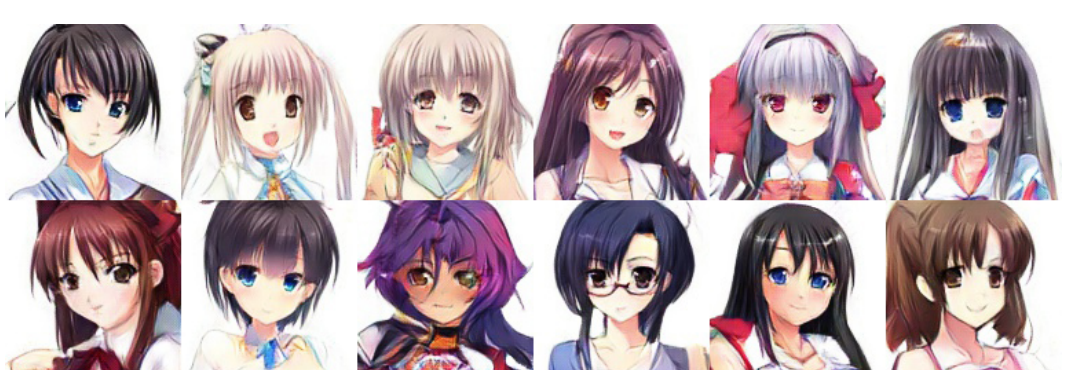
\includegraphics[width=0.8\linewidth]{animecharacter.png}
        \caption{GAN generated anime characters}
    \end{figure} 

    \subsection{CycleGAN}
    Cross-domain transfer GANs will be likely the first batch of commercial applications. These GANs transform images from one domain to another domain.
    (For example, it can transform pictures between zebras and horses.
    \begin{figure}[h]
        \centering
        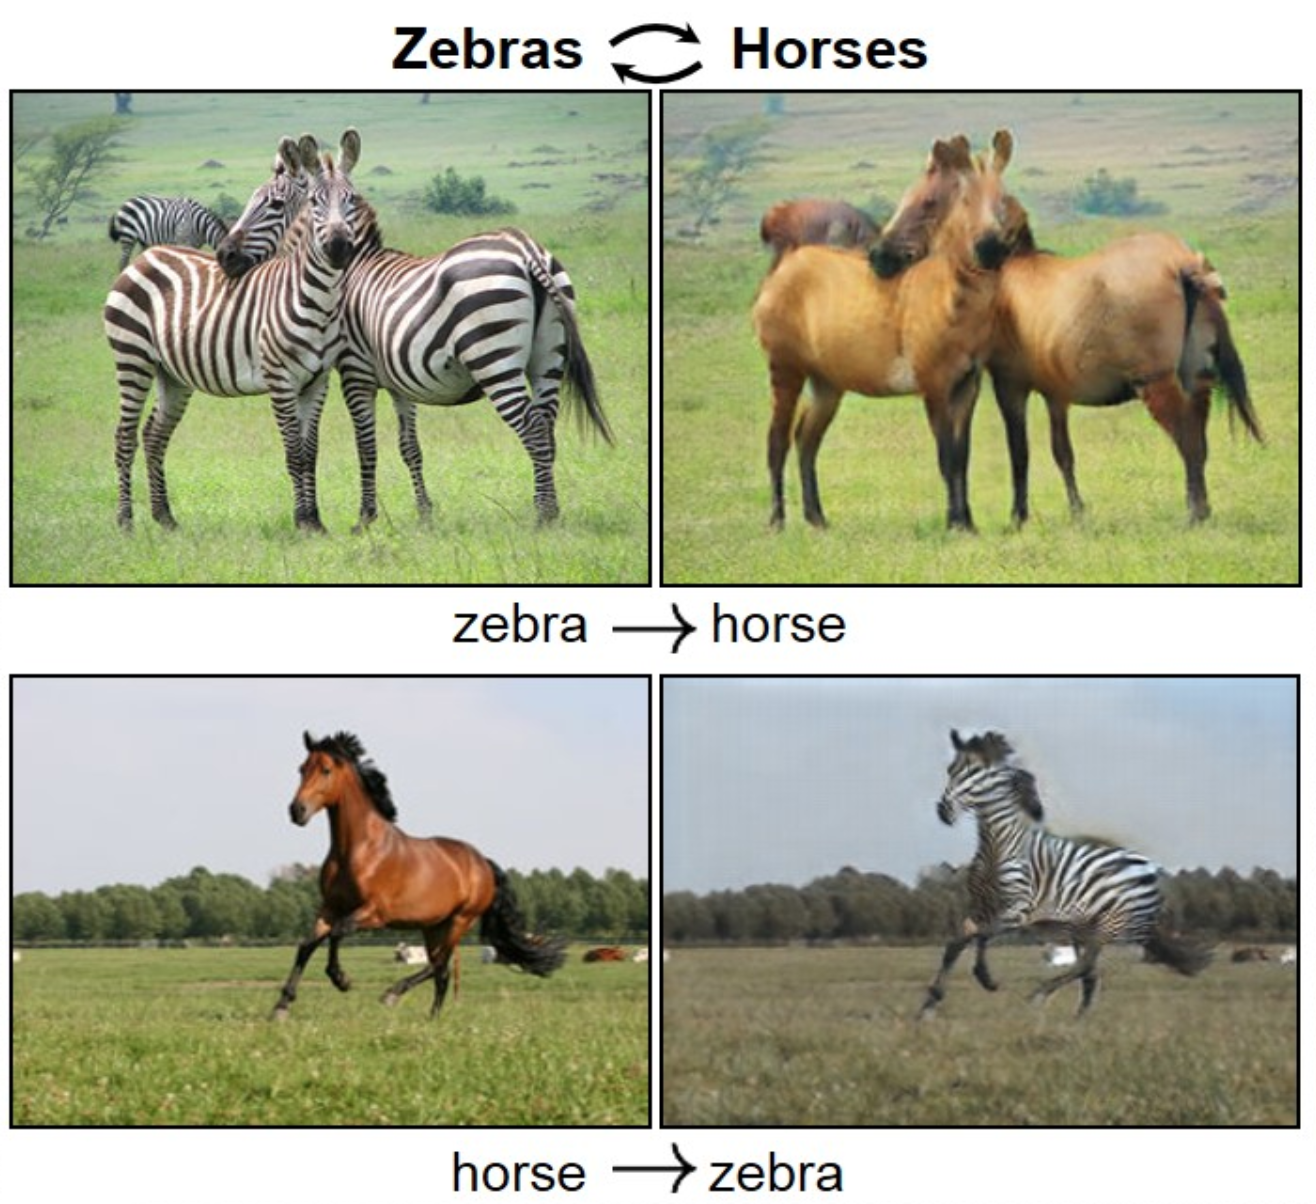
\includegraphics[width=0.5\linewidth]{zebratohorse.png}
        \caption{CycleGAN horse to zebra}
    \end{figure} 
    
    \subsection{PixelDTGAN}
    Suggesting merchandise based on celebrity pictures has been popular for fashion blogger and e-commerce. PixelDTGAN creates clothing images and styles from an image.
    \begin{figure}[h]
        \centering
        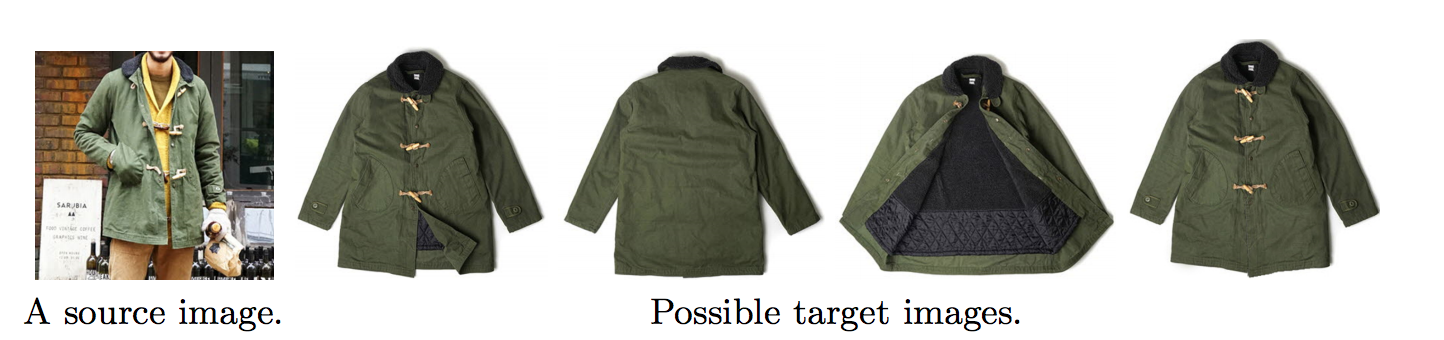
\includegraphics[width=0.9\linewidth]{pixeldtgan.png}
        \caption{PixelDTGAN}
    \end{figure} 
    
    \subsection{Super resolution}
    Create super-resolution images from the lower resolution. This is one area where GAN shows very impressive result with immediate commercial possibility.
    \begin{figure}[h]
        \centering
        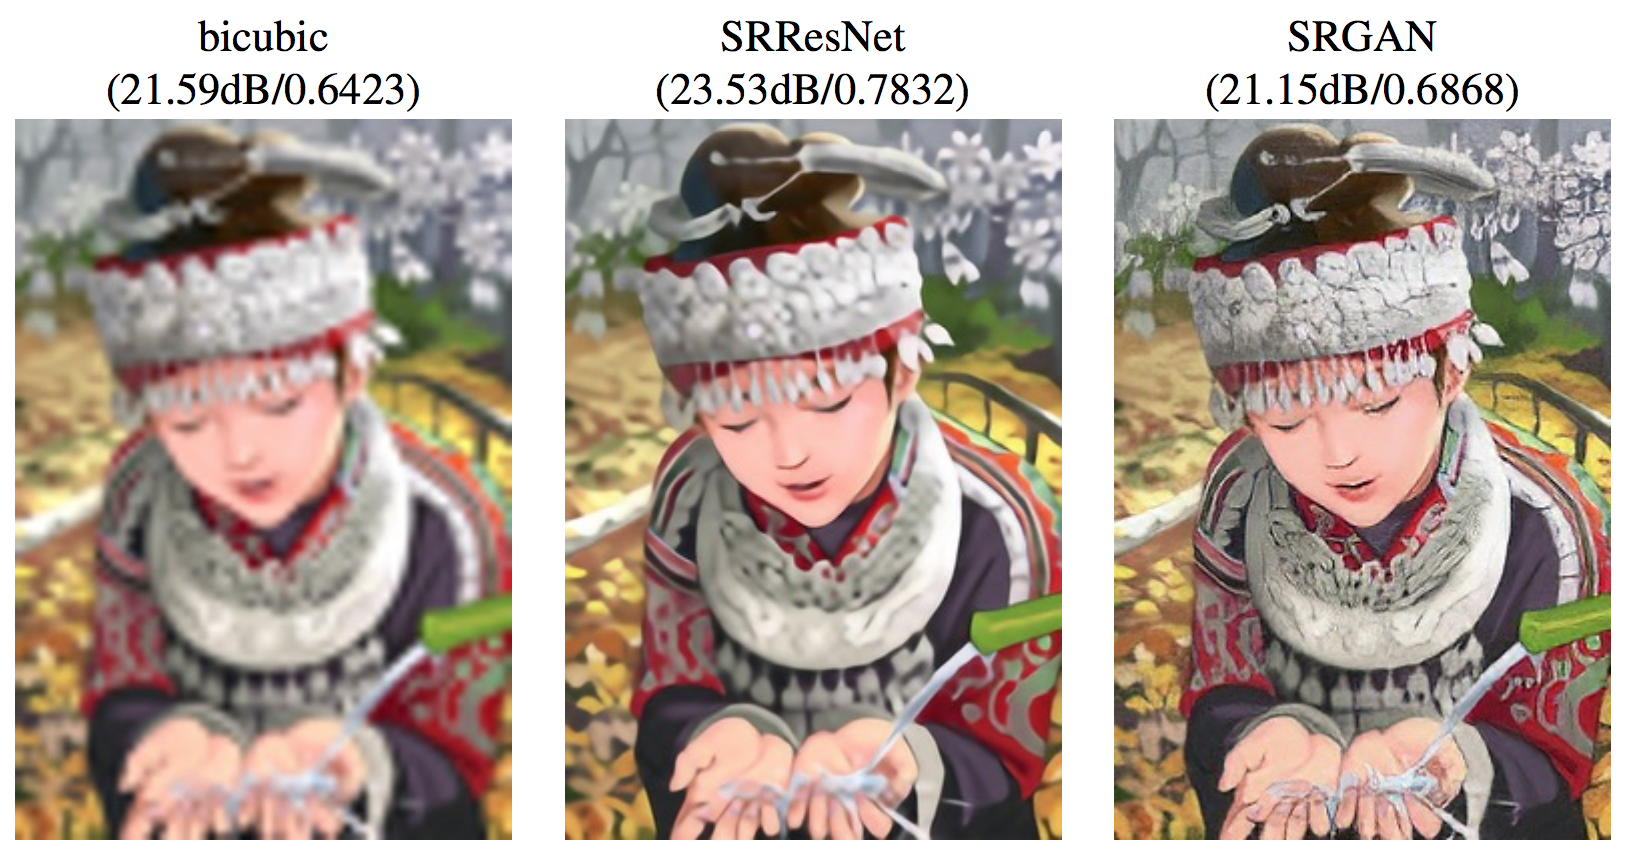
\includegraphics[width=0.8\linewidth]{superresolution.png}
        \caption{SuperResolution using GAN}
    \end{figure} 


\end{onehalfspace}

